\documentclass{article}
\usepackage{graphicx}
\usepackage[utf8]{inputenc}
\usepackage[T1]{fontenc}
\usepackage{fouriernc}
\usepackage[margin=1in]{geometry}
\usepackage{amsmath}
\DeclareUnicodeCharacter{2212}{-}
\begin{document}

\begin{titlepage}
	\centering 
	\scshape
	\vspace*{\baselineskip}
	\rule{\textwidth}{1.6pt}\vspace*{-\baselineskip}\vspace*{2pt}
	\rule{\textwidth}{0.4pt} 
	\vspace{0.75\baselineskip}
	
	{\Large CS 374 : Computational and Numerical Methods \\\vspace{0.75\baselineskip} Assignment 1 - Set 1}
	\vspace{0.75\baselineskip}
	
	\rule{\textwidth}{0.4pt}\vspace*{-\baselineskip}\vspace{3.2pt} 
	\rule{\textwidth}{1.6pt}
	
	\vspace{2\baselineskip}  
	%Title
	
	\vspace*{3\baselineskip}
	%Subtitle
	
	\vspace{0.5\baselineskip} %originally 0.5
	
	{\scshape\large Purvil Mehta (201701073) \\ Bhargey Mehta (201701074) \\} 
	
	\vspace{1\baselineskip} 
	
	\textit{Dhirubhai Ambani Institute of Information and Communication Technology \\ Gandhinagar\\} 
	\vspace*{2\baselineskip}
	\today


\end{titlepage}

\newpage
\tableofcontents
\newpage
	
\section{Logarithmic and Exponential Functions}
With the help of a single code, plot the following functions:
\begin{itemize}
    \item $y = e^x$
    \item $y = x$
    \item $y = ln(x)$
\end{itemize}
Use suitable ranges of x for each of the functions and judge their properties on various scales of x. Extending this exercise, plot $e^{\pm x}$ on the same graph and compare them.
\subsection{Plots}

\begin{figure}[!h]
    \centering
    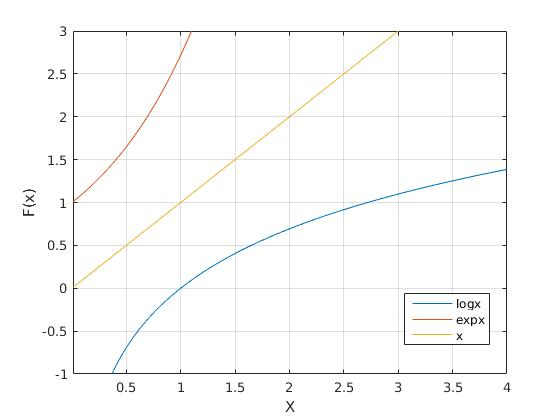
\includegraphics[scale = 0.4]{2}
    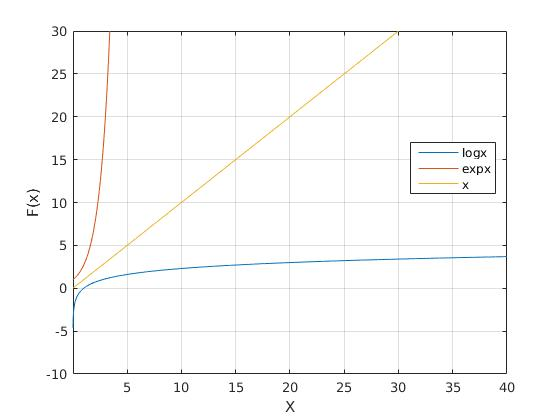
\includegraphics[scale = 0.4]{3}
    \caption{Behaviour of Functions over different ranges}
    \label{fig:ques1}
\end{figure}

\subsection{Observations}
\begin{itemize}
    \item Analytic observation shows that the plot of $\ln{x}$ would not enter the negative portion of the X-axis hence bounding the area of interest to the first and fourth quadrants only. Again the plot of $e^x$ would never enter the negative portion of Y-axis. This reduces our area of interest to the first quadrant only.
    \item We also note that the $\ln{x}$ function crosses the X-axis on $x = 0$ and the $e^{x}$ function crosses Y-axis on $y = 0$.
    \item Initial plots over the range of $[0, 4]$ give us a hint that the functions are monotonic without any turning point. To confirm it mathematically, we have the derivatives of the functions as:
    \begin{itemize}
        \item $\frac{\mathrm{d}}{\mathrm{d}x} e^x = e^x$ (Equals to zero as $x \to \infty$ And Hence no turning point)
        \item $\frac{\mathrm{d}}{\mathrm{d}x} x = 1$
        \item $\frac{\mathrm{d}}{\mathrm{d}x} \ln{x} = \frac{1}{x}$ {Equals to zero as $x \to -\infty$ And hence no turning point.}
    \end{itemize}
    \item Plots indicate that as $x$ increases, $\ln{x}$ shows very little increase and it's polar opposite $e^x$ explodes.
    \item The above fact is also seen mathematically since as $x \to \infty$, $\frac{1}{x}$ becomes small. Rate of increase of function becomes slower and slower. And similarly as $x \to \infty$, $e^x$ becomes large. Rate of increase of function becomes faster and faster and hence it explodes.
    \item $y = x$ increases with a constant rate. Hence $\forall x$,  $e^x > x > \ln{x}$
\end{itemize}
\newpage
\subsection{Comparing $e^x$ and $e^{-x}$}
\begin{figure}[!h]
    \centering
    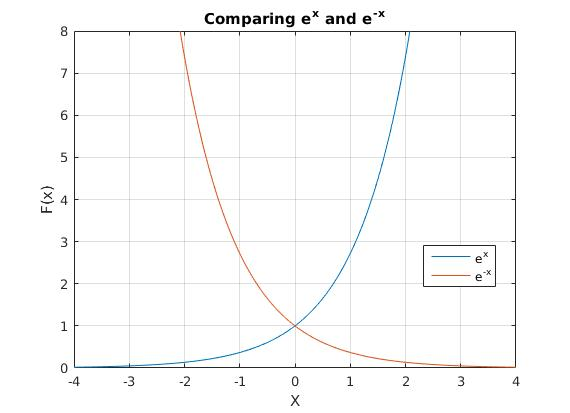
\includegraphics[scale = 0.4]{4}
    \caption{$e^x$ and $e^{-x}$}
    \label{fig:e+-x}
\end{figure}
\begin{itemize}
    \item We have already concluded that we are interested in the first and second quadrant only. 
    \item We can see that we can transform one function to the other by replacing $x$ with $-x$. The graphical interpretation of this statement is that whatever is the behaviour of one function is on going in one direction along the X-axis, the same behaviour is valid for the other function but in the opposite direction.
    \item On plotting the functions, we see that they are indeed mirror reflections of each other around the Y-axis. This mirror tends to be on the Y-axis since $x = 0$ for this line. And $x = -x$ only when $x = 0$.
    \item Using the above mirror property, we conclude that as $x \to \infty$, $e^{-x} \to 0$ because of the fact that as $x \to -\infty$, $e^x \to 0$. We have the mirror behaviour for $x \to -\infty$ as well.
\end{itemize}

\newpage
\section{Scaling of Independent Variables}
For a fixed parameter $k$, plot the function $y = \sin{kx}$ for a few suitably chosen values of $k$. What is the role of $k$ in determining the profile of the function? Thereafter, for $k = 1$, plot $\sin{x}$ and $\sin^{2}{x}$ on the same graph within $-\pi < x < \pi$ Compare both.

\subsection{Plots}
\begin{figure}[!h]
    \centering
    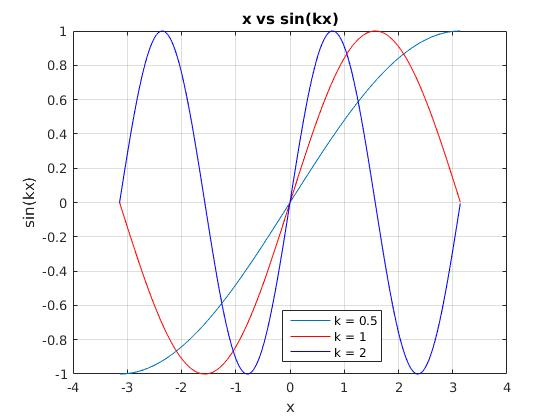
\includegraphics[scale = 0.4]{5}
    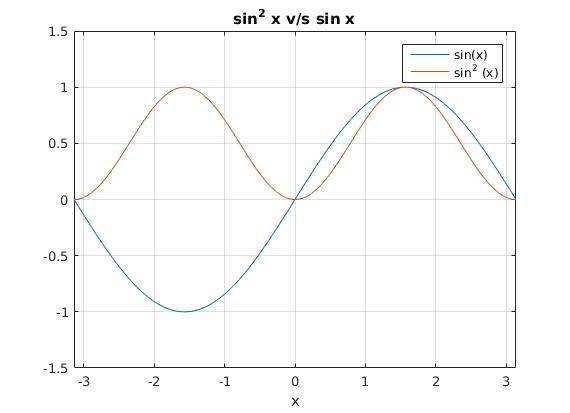
\includegraphics[scale = 0.4]{5point5.jpg}
    \caption{a) $\sin{kx}$ for $k = \frac{1}{2}, 1, 2$ and b) $\sin{x}$ vs $\sin^2{x}$}
    \label{fig:sinx}
\end{figure}

\subsection{Observations}
\subsubsection{Varying Parameter $k$}
\begin{itemize}
    \item Let's assume the point of view of the function. Whatever value $x$ assumes, it gets amplified (or attenuated) according to the parameter $k$. We can get an intuitive sense that when the inputs are appearing with $k$ times the speed, the function has to exhibit it's behaviour in a smaller period. \item Hence as $k$ increases, we see that more and more cycles of $\sin{x}$ are getting accommodated in the same period. As $k$ becomes less than 1, the reverse phenomenon occurs because now the function has to exhibit it's behaviour over a longer period. The overall effect of the parameter $k$ is thus the stretching and squeezing of the function.
\end{itemize}

\subsubsection{$\sin{x}$ vs $\sin^2{x}$}
\begin{itemize}
    \item We observe that the maximum and minimum value of the $\sin{x}$ doesn't change on squaring. They still remain 1 and 0 respectively.
    \item However since a square is always positive, it is natural for $\sin^2{x}$ to stay above or on X-axis at all times. Also square of a number smaller than 1 is smaller than the number itself, hence $\forall x \notin \{ n\frac{\pi}{2}, n\pi$ \}, we see that $\sin^2{x} < \sin{x}$ because for these $x$, $0 < \sin{x} < 1$.
    \item Since $\sin^2{x}$ is a continuous function, the derivatives exist at $x = n\pi$ and hence the function is smooth around these points. If we compare it to $y = |\sin{x}|$, it is not the case.
\end{itemize}

\newpage
\section{The Gaussian Function}
Plot the Gaussian function $y = y_0e^{-a(x-\mu)^2}$ for a few suitably chosen values of the fixed parameters $y_0$, $a$ and $\mu$. Examine the shifting profile of the function, with changes in the parameters ($\mu = vt$ simulates a single wave pulse, like a tsunami, travelling with a velocity $v$). Then for $y_0 = a = 1$ and $\mu = 0$, consider a first-order expansion of the Gaussian function to obtain the Lorentz function. Plot both of them together and compare their behaviour. For every value of x take the difference between the two functions and plot it against $x$ over $0 < x < 10$.

\subsection{Plots}
\begin{figure}[!h]
    \centering
    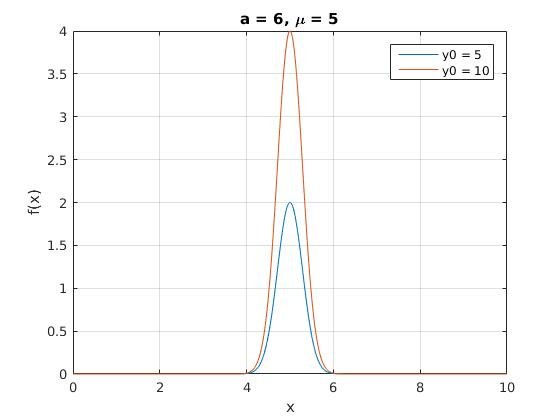
\includegraphics[scale = 0.4]{6}
    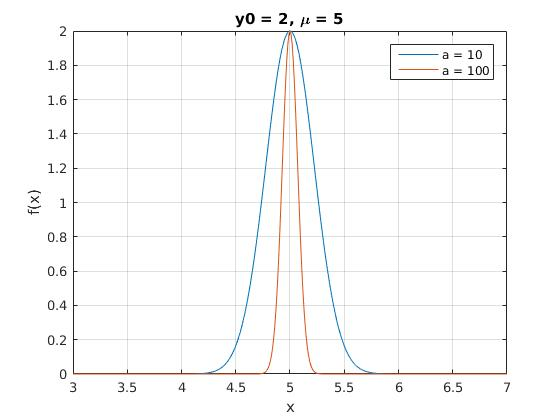
\includegraphics[scale = 0.4]{7}
    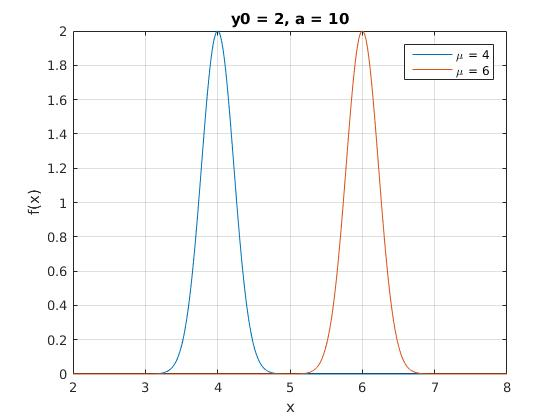
\includegraphics[scale = 0.4]{8}
    \caption{Varying different parameters of $y$}
    \label{fig:gaussian}
\end{figure}

\subsection{Observations}
\subsubsection{$y_0$ - The Amplitude Parameter}
The amplitude parameter controls how high the peak is for the Gaussian curve. Higher the amplitude parameter, higher the peak. It is independent of the mean and the variance. The value of $x$ at which these peaks occur remains the same if $\mu$ is same.

\subsubsection{$a$ - The Variance Parameter}
The Variance parameter $a$ controls informally the spread of the Gaussian curve. The higher $a$ is, the more wide is the Gauss curve. This happens because when we look at the derivative of the function, we see that
$$\frac{\mathrm{d}y}{\mathrm{d}x} = [-2a(x-\mu)][y_0e^{-a(x-\mu)^2}] = -2a(x-\mu)y$$
Thus at any point x, if $\mu$ is fixed then the rate of change is directly proportional to $-a$. If $a$ is large, $-a$ is small and so the rate of change is also small. This means the function takes more time (or X-axis values) to reach the peak and also to come down from the peak. This means the function get wider and wider as $a$ increases.

\subsubsection{$\mu$ - The Mean Parameter}
This parameter controls the position of the peak of the Gaussian curve. Shifting $\mu$ to some $\mu = \mu_1$ shifts the position of the curve to $\mu_1$. The variance and amplitude remain the same.

\flushleft
We conclude that the three parameters, $y_0, a, \mu$ independently control the behaviour of the particular Gaussian curve under consideration.

\subsection{The Lorentz Function}
The Lorentz function is the first order approximation of the Gaussian curve. We have $$y_G = \frac{1}{1+\frac{x^2}{1!}+\frac{x^4}{2!}+\frac{x^6}{3!}+...}$$
$$y_L = \frac{1}{1+x^2}$$

\begin{figure}[!h]
    \centering
    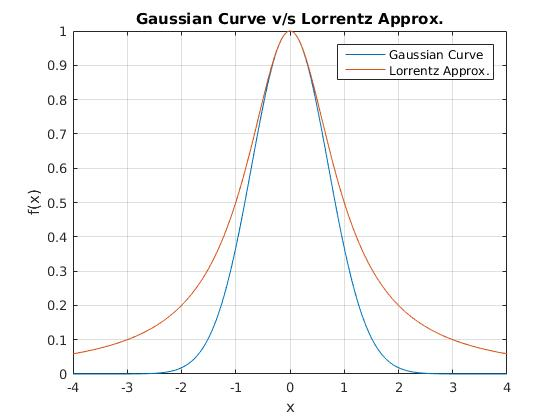
\includegraphics[scale = 0.4]{9}
    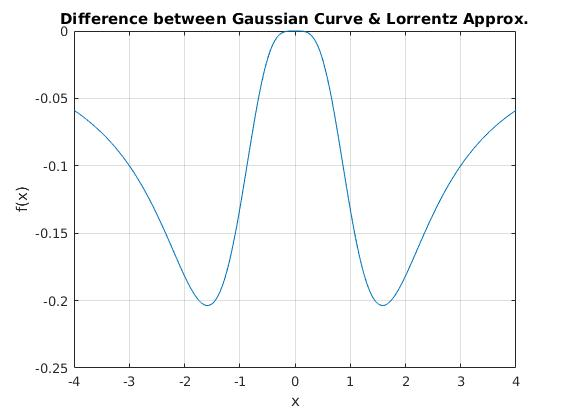
\includegraphics[scale = 0.4]{10}
    \caption{Lorentz Function and its difference with the Gaussian Function}
    \label{fig:my_label}
\end{figure}

\begin{itemize}
    \item We notice that the Lorentz function is actually missing terms in the denominator. Because of this reason, Lorentz function remains greater than the Gaussian function since the denominator is less than the same for the Gauss curve for some value of $x$.
    \item However as $x \to \infty$ or $x \to -\infty$ both the functions approach 0. Hence the $\delta y = y_G - y_L \to 0$ for the extreme cases.
    \item We also notice from the graph that as it approaches to zero the error between Lorentz Function and Gaussian Function decreases and thus in the second figure we got almost zero difference at $0$.As we move towards $x \to \infty$ or $x \to -\infty$ the margin slight increases and finally for large $x$ it merges to zero and we got two dip around small values of $x$.
\end{itemize}

\newpage
\section{Function $y = x\ln{x}$}
Plot $y = x\ln{x}$ and carefully examine it for $0 < x < 2$. Provide an analytic justification for what you observe. Also note the growth of the function for very large $x$.

\subsection{Plots}
\begin{figure}[!h]
    \centering
    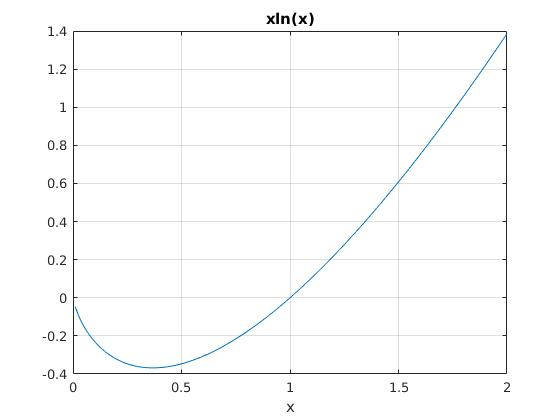
\includegraphics[scale = 0.4]{11.jpg}
    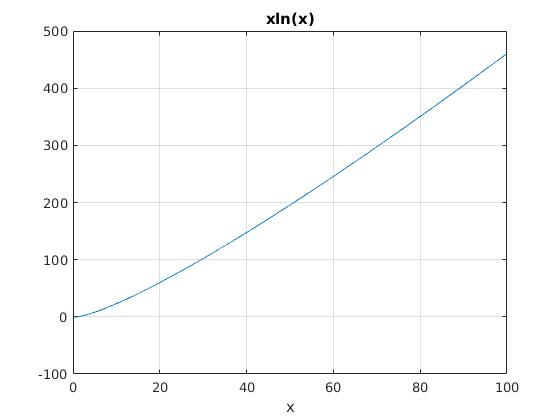
\includegraphics[scale = 0.4]{12.jpg}
    \caption{$y = x\ln{x}$}
    \label{fig:xlnx}
\end{figure}

\subsection{Observations and Justifications}
\begin{itemize}
    \item Since $\ln{x}$ cannot admit negative values as its argument, we are bound to observing the first and fourth quadrant only.
    \item We have $\frac{\mathrm{d}y}{\mathrm{d}x} = 1+\ln{x}$
    \item Setting $\frac{\mathrm{d}y}{\mathrm{d}x} = 0$ we have one turning point at $x = \frac{1}{e}$ and since $\frac{\mathrm{d^2}y}{\mathrm{d}x^2} = \frac{1}{x} > 0$, we have a minima.
    \item From our discussion in Section 1, we know that $\frac{\mathrm{d}}{\mathrm{d}x} \ln{x} = \frac{1}{x}$. So at very large $x$ the rate of change of $y = x\ln{x}$ is very slow. It becomes so small, that the function itself i.e. $\ln{x}$ can be considered constant for a significantly large interval of $x$.
    \item Using the above observation we can see that the function $y = x(\ln{x})$ assumes the form of $y = x(m) = mx$ where $m$ is a constant. This is nothing but the equation of a line. The plot thus shows a somewhat linear behaviour for large values of $x$.
    
\end{itemize}

\newpage
\section{Plot of Polynomial Function}
Plot $y(x)$, $y'(x)$ and $y''(x)$ for the following polynomial functions:
\begin{itemize}
    \item $y$ = $-ax + x^{3}$.
    \item $y = −ax^{2} + x^{4}$.
\end{itemize}
Change a continuously over a suitable range of values a$\leq$0 to observe the shift in the function profiles and their two derivatives. Carefully check all conditions for a = 0.

\subsection{Polynomial with degree three $y$ = $-ax + x^{3}$}
\subsubsection{Plots}

\begin{figure}[!h]
    \centering
    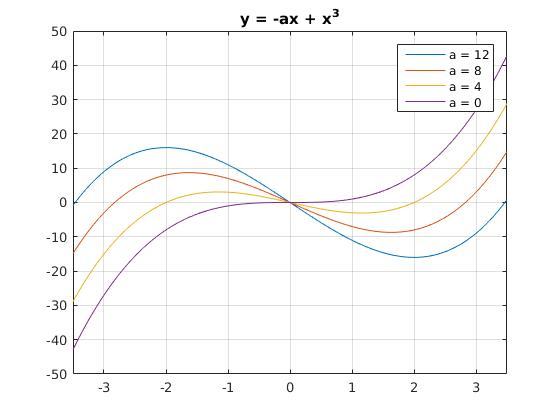
\includegraphics[scale = 0.40]{13.jpg}
    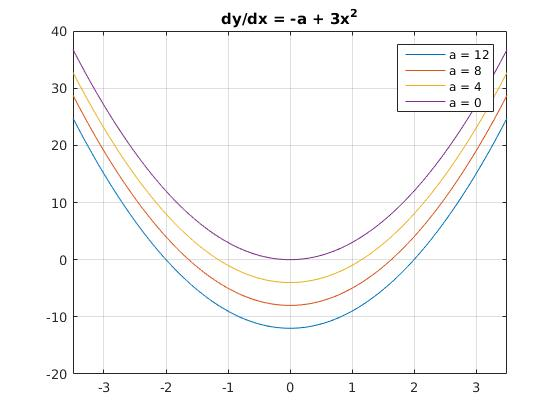
\includegraphics[scale = 0.40]{14.jpg}
    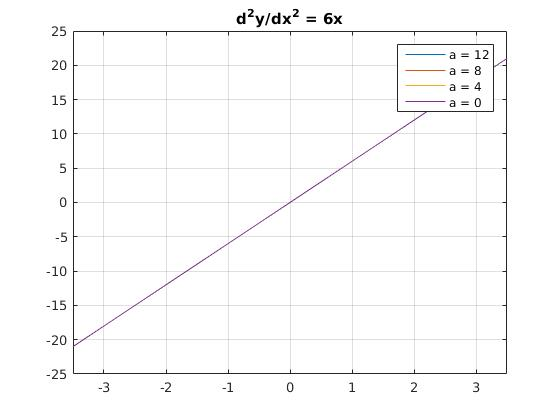
\includegraphics[scale = 0.5]{15.jpg}
    \caption{$y$ = $-ax + x^{3}$}
    \label{fig:y = -ax + x^{3}}
\end{figure}
\newpage
\subsubsection{Observations and Justifications}
\begin{itemize}
    \item Since $y$ = $-ax + x^{3}$ is cubic function, graph for the function lies in all quadrant.When $a=0$ the function will be $x^3$ and thus we get the graph as shown in figure 7.1 as purple line.  
    \item We have $\frac{\mathrm{d}y}{\mathrm{d}x} = -a + 3x^2$. So this equation is nothing but shifted parabola and exactly that is what we get in figure 7.2 having offset of $-a$.
    \item Setting $\frac{\mathrm{d}y}{\mathrm{d}x} = 0$ we have two turning point at $x = \pm\sqrt{\frac{a}{3}}$ and since $\frac{\mathrm{d^2}y}{\mathrm{d}x^2} .= 6x$, we have a minima at $x = \sqrt{\frac{a}{3}}$ and maxima at $x = \sqrt{\frac{a}{3}}$.
    \item When we set $a = 0$ maxima and minima get merged at $ x = 0$ and we get the graph as $x^3$.
    \item Since the second derivative is $6x$ which is not depend upon $a$, we get same straight line for different values of $a$.
    
\end{itemize}
\subsection{Polynomial with degree four $y = −ax^{2} + x^{4}$}
\subsubsection{Plots}

\begin{figure}[!h]
    \centering
    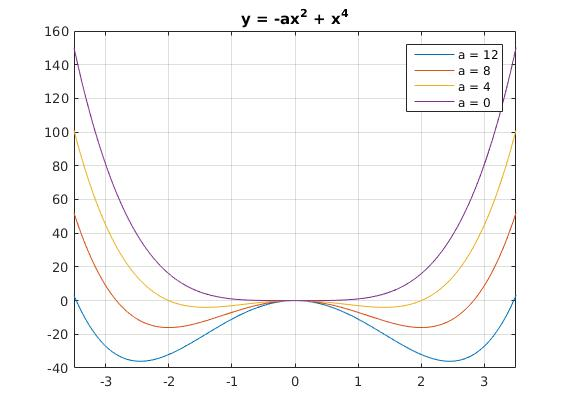
\includegraphics[scale = 0.4]{16.jpg}
    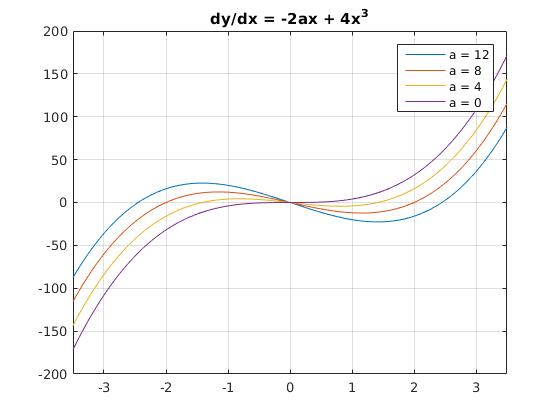
\includegraphics[scale = 0.4]{17.jpg}
    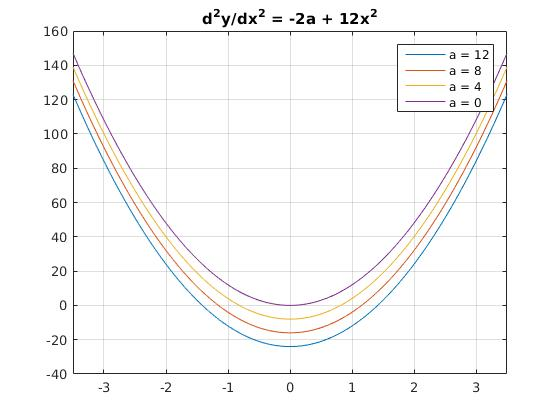
\includegraphics[scale = 0.5]{18.jpg}
    \caption{$y = −ax^{2} + x^{4}$}
    \label{fig : y = −ax^2 + x^4}
\end{figure}

\subsubsection{Observations and Justifications}
\begin{itemize}
    \item Since $y = −ax^{2} + x^{4}$ is Quartic function, graph for the function lies in all quadrant.When $a=0$ the function will be $x^4$ and thus we get the graph as shown in figure 7.1 as purple line.  
    \item We have $\frac{\mathrm{d}y}{\mathrm{d}x} = -2ax + 4x^3$. So this equation is nothing but the same we derived for the cubic equation in figure 7.
    Since it follows above cubic function, we also observed that the minima and maxima in first derivative of this function is exactly same as the zeroth derivative of cubic function. 
    \item Setting $\frac{\mathrm{d}y}{\mathrm{d}x} = 0$ we have three turning point at $x = \pm\sqrt{\frac{a}{2}}$ and $x = 0$ and since $\frac{\mathrm{d^2}y}{\mathrm{d}x^2} .= -2a + 12x^2$, we have two minimas at $x = \pm\sqrt{\frac{a}{2}}$ and maxima at $x = 0$.Exactly this kind of behaviour we got in figure 8.1. Since higher order is 4 in the equation, for large value of x it approaches to infinity in the negative and positive direction.
    \item When we set $a = 0$ maxima and two minimas get merged at $ x = 0$ and we get the graph as $x^2$.
    \item Since the second derivative is quadratic function we got shifted parabola with shift of $-a$.
    \item In the above figure 8.1, we also observed the stability of the function. When $a=0$ function is stable at $x=0$ but when we change the value of a slightly positive, then function become unstable at $x = 0$. This kind of function shows us \textbf{"Instant Change in Stability"}.
\end{itemize}
	
\end{document}